\documentclass[12pt]{article}
\usepackage{geometry}
\usepackage{fancyhdr}
\usepackage{setspace}
\usepackage{amsmath}
\usepackage{amssymb}
\usepackage{enumitem}
\usepackage{tikz}
\usetikzlibrary{automata,positioning,arrows}

\geometry{margin=1in}
\setstretch{1.1}

\begin{document}

\begin{center}
    \vspace*{0.5cm}
    {\LARGE \textbf{Homework 2}}\\[1em]
\end{center}

\noindent\textbf{Student:} \underline{\makebox[5cm][l]{Joy Jin}} \hfill
\textbf{Score:} \underline{\makebox[3cm][l]{}}

\vspace{1.5em}

\noindent\textbf{Description}

\noindent The goal of this assignment is to improve your understanding of \textbf{lexical analysis} and \textbf{derivations}.

\vspace{1em}

\noindent\textbf{Due Date}

\noindent Thursday, 10/16/2025 11:59 PM

\vspace{1.5em}
\hrule
\vspace{1em}

\noindent\textbf{[35 Points] Question 1: Regular Expression-to-Automaton}

\noindent For each of the regular expressions, construct a deterministic finite automaton (DFA). You will provide both the diagram and table representations for the DFA. You must show all the steps from generating a nondeterministic finite automaton (NFA) to a DFA. To receive full credit, you must show \textit{all} the workouts of DFA construction (i.e., Move(A, a), $\varepsilon$-closures, etc).

\vspace{1em}
\noindent\textbf{Regular Expressions:}

\begin{enumerate}[label=\arabic*.]
    \item[1.] [5 Points] $(a|b)^*$

% Disclaimer: Generated by ChatGPT from my drawing, and heavily edited (ChatGPT always screw tikz up in single-shot, and can't correct itself 50% of the time...) It's so much work that I just decided to do it myself for later problems.
    
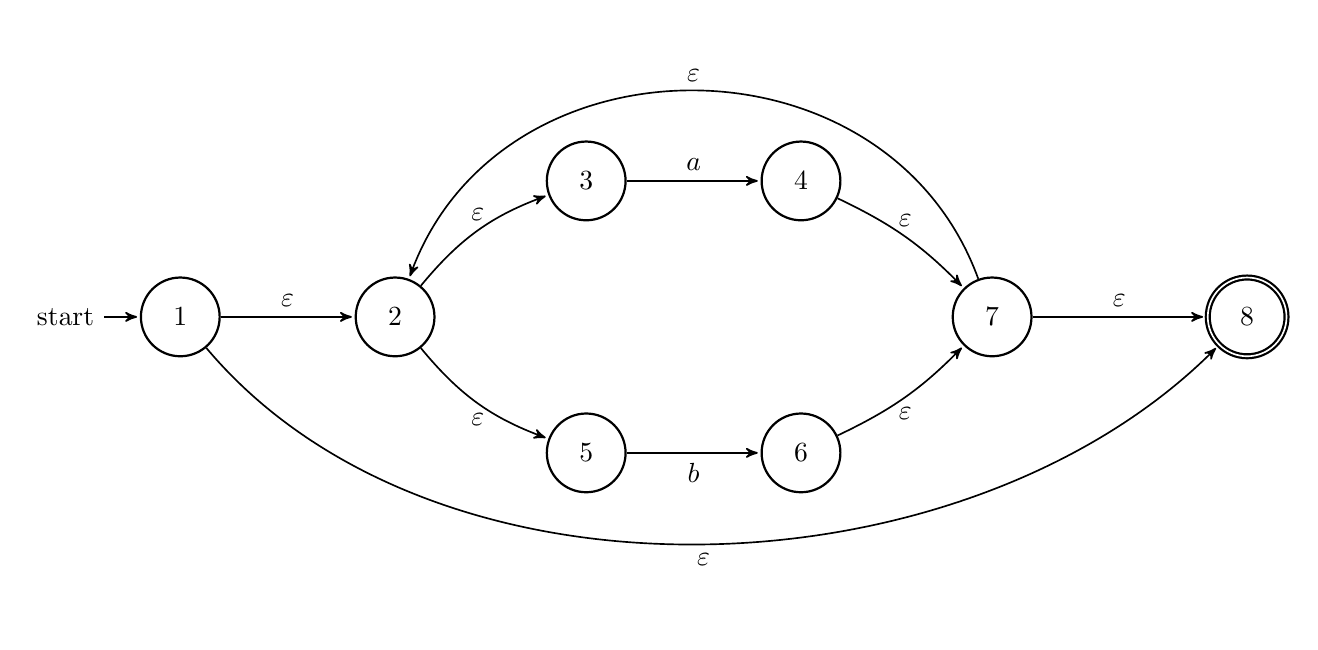
\begin{tikzpicture}[>=stealth',shorten >=1pt,auto,node distance=1.6cm,semithick]
  \tikzstyle{every state}=[draw=black,thick,minimum size=10mm]

  %--- States (numbers only, reordered) ---
  \node[state, initial] (q1) {$1$};                                     % s
  \node[state]           (q2) [right=1.7cm of q1] {$2$};                 % p0
  \node[state]           (q3) [above right=1.0cm and 1.7cm of q2] {$3$}; % p1
  \node[state]           (q4) [right=1.7cm of q3] {$4$};                 % p3
  \node[state]           (q5) [below right=1.0cm and 1.7cm of q2] {$5$}; % p2
  \node[state]           (q6) [right=1.7cm of q5] {$6$};                 % p4
  \node[state]           (q7) [below right=1.0cm and 1.7cm of q4] {$7$}; % p5
  \node[state, accepting](q8) [right=2.2cm of q7] {$8$};                 % t

  %--- Transitions ---
  \path[->]
    % from start (1)
    (q1) edge node[above] {$\varepsilon$} (q2)
    % bottom arc: start -> accepting (goes under)
    (q1) edge[out=310, in=225, looseness=.9] node[below] {$\varepsilon$} (q8)

    % split on epsilon at 2
    (q2) edge[bend left=15]  node[above] {$\varepsilon$} (q3)
    (q2) edge[bend right=15] node[below] {$\varepsilon$} (q5)

    % labeled moves
    (q3) edge node[above] {$a$} (q4)
    (q5) edge node[below] {$b$} (q6)

    % join via epsilon to 7
    (q4) edge[bend left=10]  node[above] {$\varepsilon$} (q7)
    (q6) edge[bend right=10] node[below] {$\varepsilon$} (q7)

    % loop back epsilon: 7 -> 2 (drawn above everything)
    (q7) edge[bend left=-70, looseness=1.2] node[above] {$\varepsilon$} (q2)

    % to accepting on right
    (q7) edge node[above] {$\varepsilon$} (q8);
\end{tikzpicture}\\
\begin{align}
	\epsilon\text{-closure}(1)=\{1,2,3,5,8\}:A
	\\
	\epsilon\text{-closure}(\text{move}(A,a))=\epsilon\text{-closure}(\{4\})=\{2,3,4,5,7,8\}:B
	\\
	\epsilon\text{-closure}(\text{move}(A,b))=\epsilon\text{-closure}(\{6\})=\{2,3,5,6,7,8\}:C
	\\
	\epsilon\text{-closure}(\text{move}(B,a))=\epsilon\text{-closure}(\{4\})=B
	\\
	\epsilon\text{-closure}(\text{move}(B,b))=\epsilon\text{-closure}(\{6\})=C
	\\
	\epsilon\text{-closure}(\text{move}(C,a))=\epsilon\text{-closure}(\{4\})=B
	\\
	\epsilon\text{-closure}(\text{move}(C,b))=\epsilon\text{-closure}(\{6\})=C
\end{align}
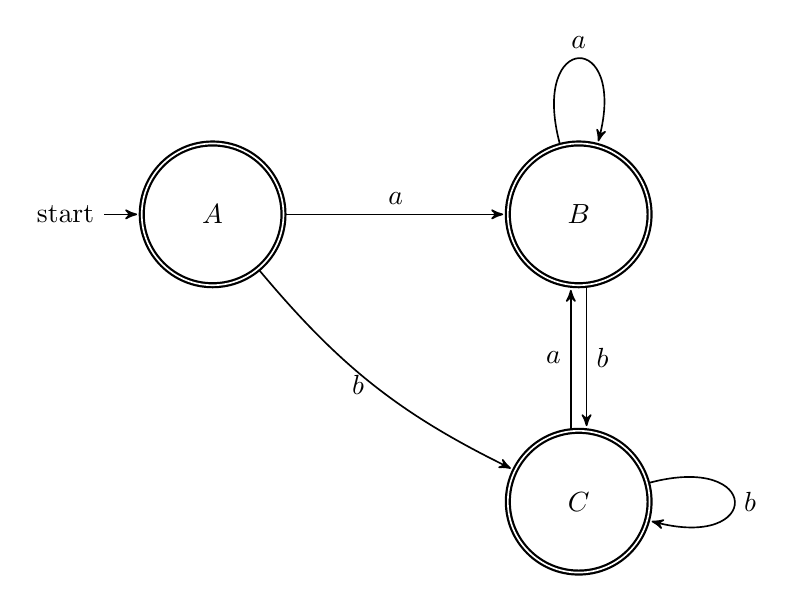
\begin{tikzpicture}[>=stealth',shorten >=1pt,auto,node distance=28mm,semithick]
  \tikzstyle{every state}=[draw=black,thick,minimum width=18mm,minimum height=10mm]

  % States
  \node[state,initial,accepting] (A) {$A$};
  \node[state,accepting] (B) [right=of A] {$B$};
  \node[state,accepting] (C) [below=18mm of B] {$C$};

  % Transitions
  \path[->]
    (A) edge[above] node{$a$} (B)
    (A) edge[bend right=12,left] node{$b$} (C)

    (B) edge[loop above] node{$a$} ()
    ([xshift=1mm]B.south) edge[right] node{$b$} ([xshift=1mm]C.north)

    ([xshift=-1mm]C.north) edge[left] node{$a$} ([xshift=-1mm]B.south)
    (C) edge[loop right] node{$b$} ();
\end{tikzpicture}

    
    \item[2.] [5 Points] $(a^*|b^*)^*$
    
    
    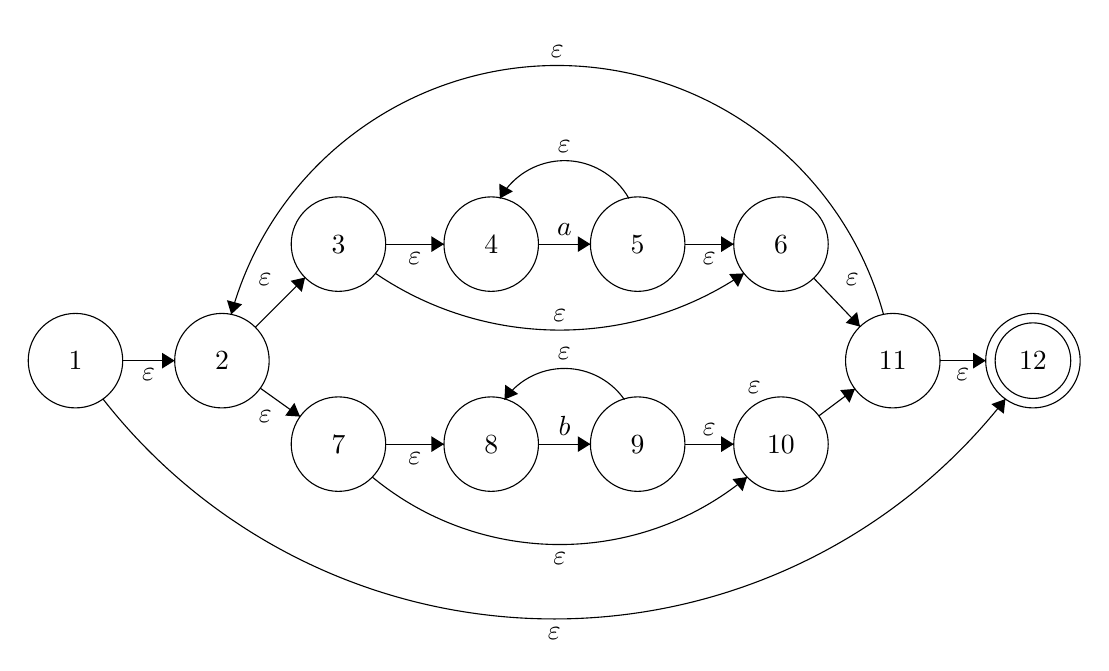
\begin{tikzpicture}[scale=0.2]
\tikzstyle{every node}+=[inner sep=0pt]
\draw [black] (3.9,-23.6) circle (3);
\draw (3.9,-23.6) node {$1$};
\draw [black] (13.2,-23.6) circle (3);
\draw (13.2,-23.6) node {$2$};
\draw [black] (20.6,-16.2) circle (3);
\draw (20.6,-16.2) node {$3$};
\draw [black] (30.3,-16.2) circle (3);
\draw (30.3,-16.2) node {$4$};
\draw [black] (39.6,-16.2) circle (3);
\draw (39.6,-16.2) node {$5$};
\draw [black] (48.7,-16.2) circle (3);
\draw (48.7,-16.2) node {$6$};
\draw [black] (55.8,-23.6) circle (3);
\draw (55.8,-23.6) node {$11$};
\draw [black] (20.6,-28.9) circle (3);
\draw (20.6,-28.9) node {$7$};
\draw [black] (30.3,-28.9) circle (3);
\draw (30.3,-28.9) node {$8$};
\draw [black] (39.6,-28.9) circle (3);
\draw (39.6,-28.9) node {$9$};
\draw [black] (48.7,-28.9) circle (3);
\draw (48.7,-28.9) node {$10$};
\draw [black] (64.7,-23.6) circle (3);
\draw (64.7,-23.6) node {$12$};
\draw [black] (64.7,-23.6) circle (2.4);
\draw [black] (6.9,-23.6) -- (10.2,-23.6);
\fill [black] (10.2,-23.6) -- (9.4,-23.1) -- (9.4,-24.1);
\draw (8.55,-24.1) node [below] {$\varepsilon$};
\draw [black] (15.32,-21.48) -- (18.48,-18.32);
\fill [black] (18.48,-18.32) -- (17.56,-18.53) -- (18.27,-19.24);
\draw (16.38,-18.42) node [left] {$\varepsilon$};
\draw [black] (23.6,-16.2) -- (27.3,-16.2);
\fill [black] (27.3,-16.2) -- (26.5,-15.7) -- (26.5,-16.7);
\draw (25.45,-16.7) node [below] {$\varepsilon$};
\draw [black] (33.3,-16.2) -- (36.6,-16.2);
\fill [black] (36.6,-16.2) -- (35.8,-15.7) -- (35.8,-16.7);
\draw (34.95,-15.7) node [above] {$a$};
\draw [black] (42.6,-16.2) -- (45.7,-16.2);
\fill [black] (45.7,-16.2) -- (44.9,-15.7) -- (44.9,-16.7);
\draw (44.15,-16.7) node [below] {$\varepsilon$};
\draw [black] (50.78,-18.36) -- (53.72,-21.44);
\fill [black] (53.72,-21.44) -- (53.53,-20.51) -- (52.81,-21.2);
\draw (52.78,-18.43) node [right] {$\varepsilon$};
\draw [black] (51.1,-27.11) -- (53.4,-25.39);
\fill [black] (53.4,-25.39) -- (52.46,-25.47) -- (53.05,-26.27);
\draw (47.01,-25.75) node [above] {$\varepsilon$};
\draw [black] (42.6,-28.9) -- (45.7,-28.9);
\fill [black] (45.7,-28.9) -- (44.9,-28.4) -- (44.9,-29.4);
\draw (44.15,-28.4) node [above] {$\varepsilon$};
\draw [black] (23.6,-28.9) -- (27.3,-28.9);
\fill [black] (27.3,-28.9) -- (26.5,-28.4) -- (26.5,-29.4);
\draw (25.45,-29.4) node [below] {$\varepsilon$};
\draw [black] (33.3,-28.9) -- (36.6,-28.9);
\fill [black] (36.6,-28.9) -- (35.8,-28.4) -- (35.8,-29.4);
\draw (34.95,-28.4) node [above] {$b$};
\draw [black] (15.64,-25.35) -- (18.16,-27.15);
\fill [black] (18.16,-27.15) -- (17.8,-26.28) -- (17.22,-27.09);
\draw (15.96,-26.75) node [below] {$\varepsilon$};
\draw [black] (58.8,-23.6) -- (61.7,-23.6);
\fill [black] (61.7,-23.6) -- (60.9,-23.1) -- (60.9,-24.1);
\draw (60.25,-24.1) node [below] {$\varepsilon$};
\draw [black] (13.788,-20.661) arc (164.67747:15.32253:21.475);
\fill [black] (13.79,-20.66) -- (14.48,-20.02) -- (13.52,-19.76);
\draw (34.5,-4.36) node [above] {$\varepsilon$};
\draw [black] (30.855,-13.304) arc (-209.1725:-330.8275:4.69);
\fill [black] (30.85,-13.3) -- (31.68,-12.85) -- (30.81,-12.36);
\draw (34.95,-10.4) node [above] {$\varepsilon$};
\draw [black] (31.141,-26.074) arc (-215.04582:-324.95418:4.653);
\fill [black] (31.14,-26.07) -- (32.01,-25.71) -- (31.19,-25.13);
\draw (34.95,-23.59) node [above] {$\varepsilon$};
\draw [black] (46.552,-30.99) arc (-50.38099:-129.61901:18.665);
\fill [black] (46.55,-30.99) -- (45.62,-31.12) -- (46.26,-31.89);
\draw (34.65,-35.78) node [below] {$\varepsilon$};
\draw [black] (62.951,-26.037) arc (-38.03054:-141.96946:36.374);
\fill [black] (62.95,-26.04) -- (62.06,-26.36) -- (62.85,-26.97);
\draw (34.3,-40.5) node [below] {$\varepsilon$};
\draw [black] (46.349,-18.059) arc (-55.78833:-124.21167:20.808);
\fill [black] (46.35,-18.06) -- (45.41,-18.1) -- (45.97,-18.92);
\draw (34.65,-21.16) node [above] {$\varepsilon$};
\end{tikzpicture}
    
    \begin{align}
	\epsilon\text{-closure}(1)=\{1,2,3,4,6,7,8,10,11,12\}:A
	\\
	\epsilon\text{-closure}(\text{move}(A,a))=\epsilon\text{-closure}(\{5\})=\{2,3,4,5,6,7,8,10,11,12\}:B
	\\
	\epsilon\text{-closure}(\text{move}(A,b))=\epsilon\text{-closure}(\{9\})=\{2,3,4,6,7,8,9,10,11,12\}:C
	\\
	\epsilon\text{-closure}(\text{move}(B,a))=\epsilon\text{-closure}(\{5\})=B
	\\
	\epsilon\text{-closure}(\text{move}(B,b))=\epsilon\text{-closure}(\{9\})=C
	\\
	\epsilon\text{-closure}(\text{move}(C,a))=\epsilon\text{-closure}(\{5\})=B
	\\
	\epsilon\text{-closure}(\text{move}(C,b))=\epsilon\text{-closure}(\{9\})=C
\end{align}

We get the same DFA, so we can use the graph earlier:

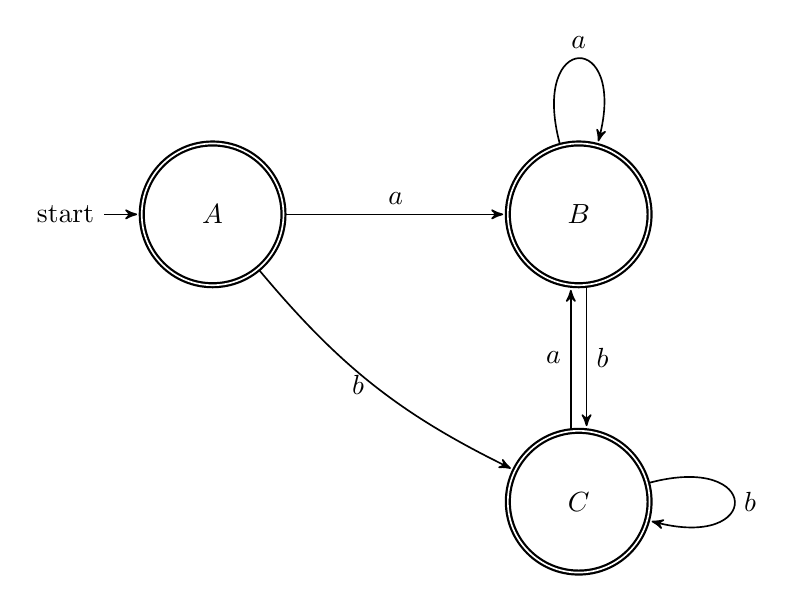
\begin{tikzpicture}[>=stealth',shorten >=1pt,auto,node distance=28mm,semithick]
  \tikzstyle{every state}=[draw=black,thick,minimum width=18mm,minimum height=10mm]

  % States
  \node[state,initial,accepting] (A) {$A$};
  \node[state,accepting] (B) [right=of A] {$B$};
  \node[state,accepting] (C) [below=18mm of B] {$C$};

  % Transitions
  \path[->]
    (A) edge[above] node{$a$} (B)
    (A) edge[bend right=12,left] node{$b$} (C)

    (B) edge[loop above] node{$a$} ()
    ([xshift=1mm]B.south) edge[right] node{$b$} ([xshift=1mm]C.north)

    ([xshift=-1mm]C.north) edge[left] node{$a$} ([xshift=-1mm]B.south)
    (C) edge[loop right] node{$b$} ();
\end{tikzpicture}
    
    
    
    
    
    \item[3.] [10 Points] $c(c|d)^*dd$
    
    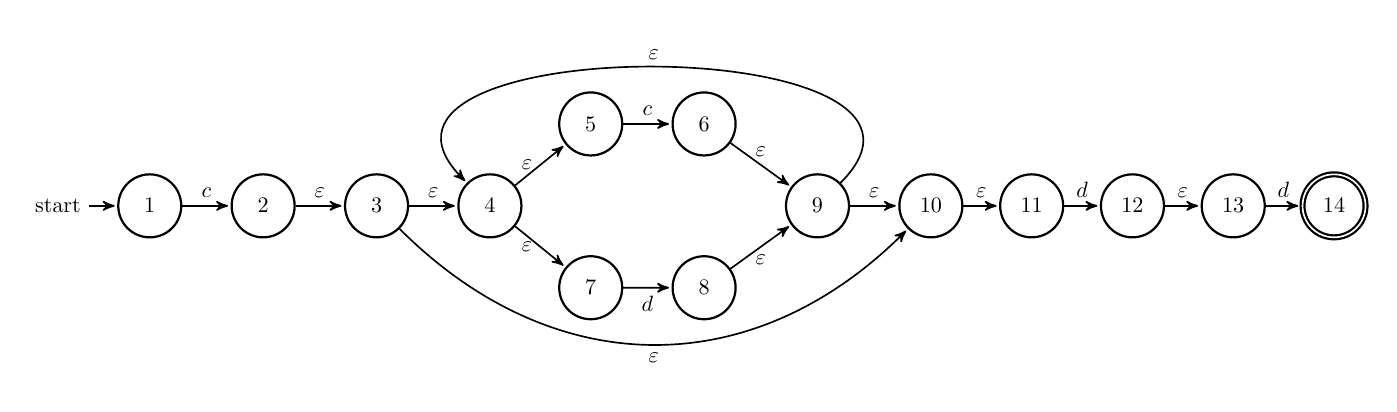
\begin{tikzpicture}[
  >=stealth',
  shorten >=1pt,
  auto,
  semithick,
  scale=0.8, transform shape, % <— scales entire diagram to fit page
  bend left/.style={out=45,in=135},
  bend right/.style={out=-45,in=-135}
]
  \tikzstyle{every state}=[draw=black,thick,minimum size=10mm]

  % Main nodes
  \node[state, initial] (q1) at (0,0) {1};
  \node[state] (q2) at (1.8,0) {2};
  \node[state] (q3) at (3.6,0) {3};
  \node[state] (q4) at (5.4,0) {4};

  % Union branches
  \node[state] (q5) at (7.0,1.3) {5};
  \node[state] (q6) at (8.8,1.3) {6};
  \node[state] (q7) at (7.0,-1.3) {7};
  \node[state] (q8) at (8.8,-1.3) {8};
  \node[state] (q9) at (10.6,0) {9};
  \node[state] (q10) at (12.4,0) {10};

  % Final dd
  \node[state] (q11) at (14.0,0) {11};
  \node[state] (q12) at (15.6,0) {12};
  \node[state] (q13) at (17.2,0) {13};
  \node[state, accepting] (q14) at (18.8,0) {14};

  % --- Edges ---
  \path[->] (q1) edge node {$c$} (q2);
  \path[->] (q2) edge node {$\varepsilon$} (q3);

  % Star entry
  \path[->] (q3) edge node[above] {$\varepsilon$} (q4);
  \path[->] (q3) edge[bend right, looseness=1.1] node[below] {$\varepsilon$} (q10);

  % Union
  \path[->] (q4) edge node[left] {$\varepsilon$} (q5);
  \path[->] (q4) edge node[left] {$\varepsilon$} (q7);
  \path[->] (q5) edge node {$c$} (q6);
  \path[->] (q6) edge node[above] {$\varepsilon$} (q9);
  \path[->] (q7) edge node[below] {$d$} (q8);
  \path[->] (q8) edge node[below] {$\varepsilon$} (q9);

  % Star loop and exit
  \path[->] (q9) edge[looseness=1.5] node[above] {$\varepsilon$} (q4);
  \path[->] (q9) edge node {$\varepsilon$} (q10);

  % Final dd
  \path[->] (q10) edge node {$\varepsilon$} (q11);
  \path[->] (q11) edge node {$d$} (q12);
  \path[->] (q12) edge node {$\varepsilon$} (q13);
  \path[->] (q13) edge node {$d$} (q14);
\end{tikzpicture}

\begin{align}
	\epsilon\text{-closure}(1)=\{1\}:A
	\notag\\
	\epsilon\text{-closure}(\text{move}(A,c))=\epsilon\text{-closure}(\{2\})=\{2,3,4,5,7,10,11\}:B
	\notag\\
	\epsilon\text{-closure}(\text{move}(A,d))=\epsilon\text{-closure}(\{\})=\{\}:C
	\notag\\
	\epsilon\text{-closure}(\text{move}(B,c))=\epsilon\text{-closure}(\{6\})=\{4, 5, 6, 7, 9, 10, 11\}: D
	\notag\\
	\epsilon\text{-closure}(\text{move}(B,d))=\epsilon\text{-closure}(\{8, 12\})=\{4, 5, 7, 8, 9, 10, 11, 12, 13\}: E
	\notag\\
	\epsilon\text{-closure}(\text{move}(C,c))=\epsilon\text{-closure}(\{\})=C
	\notag\\
	\epsilon\text{-closure}(\text{move}(C,d))=\epsilon\text{-closure}(\{\})=C
	\notag\\
	\epsilon\text{-closure}(\text{move}(D,c))=\epsilon\text{-closure}(\{6\})=D
	\notag\\
	\epsilon\text{-closure}(\text{move}(D,d))=\epsilon\text{-closure}(\{8, 12\})=E
	\notag\\
	\epsilon\text{-closure}(\text{move}(E,c))=\epsilon\text{-closure}(\{6\})=D
	\notag\\
	\epsilon\text{-closure}(\text{move}(E,d))=\epsilon\text{-closure}(\{8, 12, 14\})=\{4, 5, 7, 8, 9, 10, 11, 12, 13, 14\}:F
	\notag\\
	\epsilon\text{-closure}(\text{move}(F,c))=\epsilon\text{-closure}(\{6\})=D
	\notag\\
	\epsilon\text{-closure}(\text{move}(F,d))=\epsilon\text{-closure}(\{8, 12, 14\})=F
\end{align}

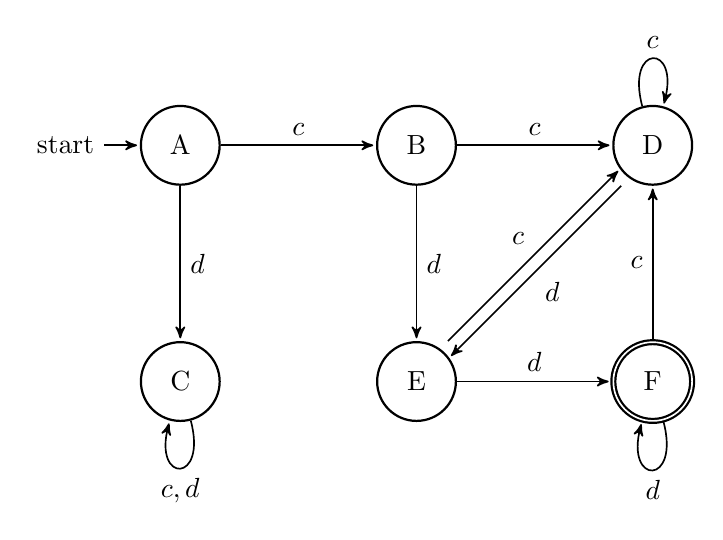
\begin{tikzpicture}[
  >=stealth',shorten >=1pt,auto,semithick,
  scale=1, transform shape
]
  \tikzstyle{every state}=[draw=black,thick,minimum size=10mm]

  % Nodes (laid out roughly left->right)
  \node[state, initial]      (D0) at (0,0)    {A};
  \node[state]               (D1) at (3,0)  {B};
  \node[state]               (D3) at (6,0)  {D};
  \node[state]               (D4) at (3,-3) {E};
  \node[state, accepting]    (D5) at (6,-3) {F};

  % Dead state beneath D1
  \node[state]               (D2) at (0,-3) {C};

  % Edges
  \path[->] (D0) edge node {$c$} (D1);
  \path[->] (D0) edge node[right] {$d$} (D2);

  \path[->] (D1) edge node {$c$} (D3);
  \path[->] (D1) edge node {$d$} (D4);

  \path[->] (D2) edge[loop below] node {$c,d$} (D2);

  \path[->] (D3) edge[loop above] node {$c$} (D3);
  
  
  
  \path[->] ([xshift=-4mm]D3.south) edge node {$d$} ([xshift=-1mm,yshift=3mm]D4.east);

  \path[->] ([xshift=4mm]D4.north) edge node {$c$} ([xshift=1mm,yshift=-3mm]D3.west);
  
  
  
  \path[->] (D4) edge node {$d$} (D5);

  \path[->] (D5) edge node {$c$} (D3);
  \path[->] (D5) edge[loop below] node {$d$} (D5);
\end{tikzpicture}

    
    \item[4.] [15 Points] $(a|b)a(a|b)b$

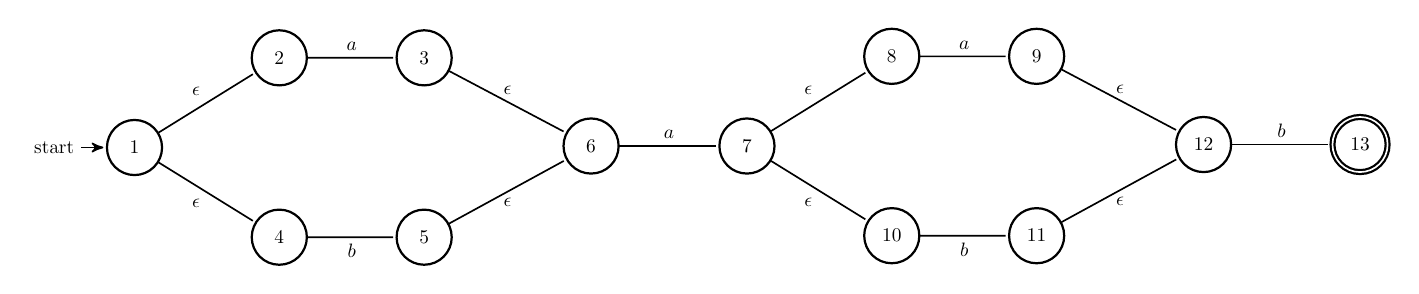
\begin{tikzpicture}[>=stealth',shorten >=1pt,auto,node distance=1.8cm,semithick,scale=0.7, transform shape,]
  \tikzstyle{every state}=[draw=black,thick,minimum size=10mm]

  % Row layout helpers
  % Left block (first (a|b))
  \node[state, initial] (q1) {1};

  \node[state] (q2) [above right=0.9cm and 1.9cm of q1] {2};
  \node[state] (q3) [right=1.6cm of q2] {3};

  \node[state] (q4) [below right=0.9cm and 1.9cm of q1] {4};
  \node[state] (q5) [right=1.6cm of q4] {5};

  \node[state] (q6) [right=2.0cm of q3, yshift=-1.6cm] {6};

  % Middle literal 'a'
  \node[state] (q7) [right=1.8cm of q6] {7};

  % Right block (second (a|b))
  \node[state] (q8) [above right=0.9cm and 1.9cm of q7] {8};
  \node[state] (q9) [right=1.6cm of q8] {9};

  \node[state] (q10) [below right=0.9cm and 1.9cm of q7] {10};
  \node[state] (q11) [right=1.6cm of q10] {11};

  \node[state] (q12) [right=2.0cm of q9, yshift=-1.6cm] {12};

  % Final 'b' and accept
  \node[state, accepting] (q13) [right=1.8cm of q12] {13};

  % Edges: first (a|b)
  \path
    (q1) edge[above left] node{$\epsilon$} (q2)
    (q1) edge[below left] node{$\epsilon$} (q4)

    (q2) edge[above] node{$a$} (q3)
    (q4) edge[below] node{$b$} (q5)

    (q3) edge[above] node{$\epsilon$} (q6)
    (q5) edge[below] node{$\epsilon$} (q6);

  % Literal 'a'
  \path (q6) edge[above] node{$a$} (q7);

  % Edges: second (a|b)
  \path
    (q7) edge[above left] node{$\epsilon$} (q8)
    (q7) edge[below left] node{$\epsilon$} (q10)

    (q8) edge[above] node{$a$} (q9)
    (q10) edge[below] node{$b$} (q11)

    (q9) edge[above] node{$\epsilon$} (q12)
    (q11) edge[below] node{$\epsilon$} (q12);

  % Final 'b'
  \path (q12) edge[above] node{$b$} (q13);
\end{tikzpicture}
Here we removed the $\varepsilon$ in concatenation to simplify.
\begin{align}
	\epsilon\text{-closure}(1)=\{1,2,4\}:A
	\\
	\epsilon\text{-closure}(\text{move}(A,a))=\epsilon\text{-closure}(\{3\})=\{3, 6\}:B
	\\
	\epsilon\text{-closure}(\text{move}(A,b))=\epsilon\text{-closure}(\{5\})=\{5, 6\}:C
	\\
	\epsilon\text{-closure}(\text{move}(B,a))=\epsilon\text{-closure}(\{7\})=\{7, 8, 10\}:D
	\\
	\epsilon\text{-closure}(\text{move}(B,b))=\epsilon\text{-closure}(\{\})=\{\}:E
	\\
	\epsilon\text{-closure}(\text{move}(C,a))=\epsilon\text{-closure}(\{7\})=D
	\\
	\epsilon\text{-closure}(\text{move}(C,b))=\epsilon\text{-closure}(\{\})=E
	\\
	\epsilon\text{-closure}(\text{move}(D,a))=\epsilon\text{-closure}(\{9\})=\{9,12\}:F
	\\
	\epsilon\text{-closure}(\text{move}(D,b))=\epsilon\text{-closure}(\{11\})=\{11,12\}=G
	\\
	\epsilon\text{-closure}(\text{move}(E,a))=\epsilon\text{-closure}(\{\})=E
	\\
	\epsilon\text{-closure}(\text{move}(E,b))=\epsilon\text{-closure}(\{\})=E
	\\
	\epsilon\text{-closure}(\text{move}(F,a))=\epsilon\text{-closure}(\{\})=E
	\\
	\epsilon\text{-closure}(\text{move}(F,b))=\epsilon\text{-closure}(\{13\})=\{13\}:H
	\\
	\epsilon\text{-closure}(\text{move}(G,a))=\epsilon\text{-closure}(\{\})=E
	\\
	\epsilon\text{-closure}(\text{move}(G,b))=\epsilon\text{-closure}(\{13\})=H
	\\
	\epsilon\text{-closure}(\text{move}(H,a))=\epsilon\text{-closure}(\{\})=E
	\\
	\epsilon\text{-closure}(\text{move}(H,b))=\epsilon\text{-closure}(\{\})=E
\end{align}
    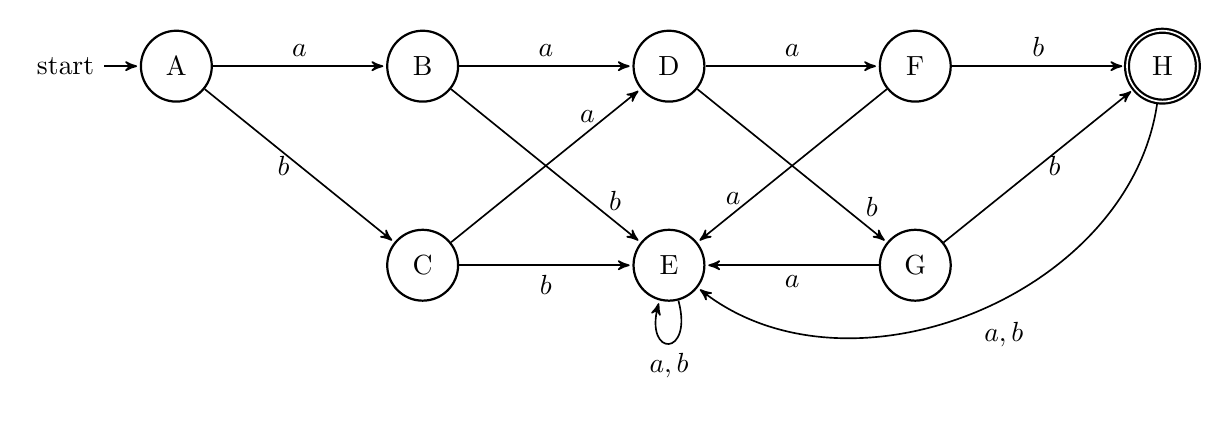
\begin{tikzpicture}[>=stealth',shorten >=1pt,auto,node distance=2.0cm,semithick]
  \tikzstyle{every state}=[draw=black,thick,minimum size=9mm]

  % States
  \node[state, initial] (A) {A};
  \node[state] (B) [right=2.2cm of A] {B};
  \node[state] (C) [below=1.6cm of B] {C};
  \node[state] (D) [right=2.2cm of B] {D};
  \node[state] (E) [below=1.6cm of D] {E};
  \node[state] (F) [right=2.2cm of D] {F};
  \node[state] (G) [below=1.6cm of F] {G};
  \node[state, accepting] (H) [right=2.2cm of F, yshift=0cm] {H};

  % Transitions
  \path[->]
    (A) edge[above] node{$a$} (B)
        edge[left]  node{$b$} (C)

    (B) edge[above] node{$a$} (D)
        edge[left, above]  node[xshift=25pt, yshift=-20pt]{$b$} (E)

    (C) edge[above] node[xshift=15pt, yshift=12pt]{$a$} (D)
        edge[left, below]  node{$b$} (E)

    (D) edge[above] node{$a$} (F)
        edge[right] node[xshift=23pt, yshift=-15pt]{$b$} (G)

    (F) edge[above] node{$b$} (H)
        edge[left] node[xshift=-15pt, yshift=-12pt]{$a$} (E)

    (G) edge[right] node{$b$} (H)
        edge[left, below] node{$a$} (E)

    (H) edge[bend left=12300] node{$a,b$} (E)

    (E) edge[loop below] node{$a,b$} ();

\end{tikzpicture}

\end{enumerate}

\newpage

\noindent\textbf{[15 Points] Question 2: Derivations}

\noindent For each of the grammar and target string, show all the steps of the leftmost and rightmost derivations. Clearly show each step.

\vspace{1em}

\begin{enumerate}[label=\arabic*.]
    \item[1.] [5 Points] Grammar: 
    \[
        S \rightarrow 0S1 \mid \epsilon
    \]
    String: $0011$
    
\begin{equation}
  S \Rightarrow 0S1 \Rightarrow 00S11 \Rightarrow 00\epsilon11 \checkmark
\end{equation}
Rightmost: identical.
    
    \item[2.] [5 Points] Grammar:
    \[
        S \rightarrow a \mid (L)
    \]
    \[
        L \rightarrow L;S \mid S
    \]
    String: $w = ((a; a); a)$
    
\begin{align}
S &\Rightarrow (L) \notag\\
  &\Rightarrow (L;S) \notag\\
  &\Rightarrow (S;S) \notag\\
  &\Rightarrow ((L);S) \notag\\
  &\Rightarrow ((L;S);S) \notag\\
  &\Rightarrow ((S;S);S) \notag\\
  &\Rightarrow ((a;S);S) \notag\\
  &\Rightarrow ((a;a);S) \notag\\
  &\Rightarrow ((a;a);a)
\end{align}
Right: 
\begin{align}
S &\Rightarrow (L) \notag\\
  &\Rightarrow (L;S) \notag\\
  &\Rightarrow (L;a) \notag\\
  &\Rightarrow (S;a) \notag\\
  &\Rightarrow ((L);a) \notag\\
  &\Rightarrow ((L;S);a) \notag\\
  &\Rightarrow ((L;a);a) \notag\\
  &\Rightarrow ((S;a);a) \notag\\
  &\Rightarrow ((a;a);a)
\end{align}



    
    \item[3.] [5 Points] Grammar:
    \[
        L \rightarrow L,E \mid E
    \]
    \[
        E \rightarrow E+E \mid id
    \]
    String: $w = id, id + id$
    
    
\begin{align}
L &\Rightarrow L, E \notag\\
  &\Rightarrow E, E \notag\\
  &\Rightarrow id, E \notag\\
  &\Rightarrow id, E + E \notag\\
  &\Rightarrow id, id + E \notag\\
  &\Rightarrow id, id + id
\end{align}
Rightmost:
\begin{align}
L &\Rightarrow L, E \notag\\
  &\Rightarrow L, E + E \notag\\
  &\Rightarrow L, E + id \notag\\
  &\Rightarrow L, id + id \notag\\
  &\Rightarrow E, id + id \notag\\
  &\Rightarrow id, id + id
\end{align}

    
    
\end{enumerate}

\end{document}
